% THIS IS SIGPROC-SP.TEX - VERSION 3.1
% WORKS WITH V3.2SP OF ACM_PROC_ARTICLE-SP.CLS
% APRIL 2009
%
% It is an example file showing how to use the 'acm_proc_article-sp.cls' V3.2SP
% LaTeX2e document class file for Conference Proceedings submissions.
% ----------------------------------------------------------------------------------------------------------------
% This .tex file (and associated .cls V3.2SP) *DOES NOT* produce:
%       1) The Permission Statement
%       2) The Conference (location) Info information
%       3) The Copyright Line with ACM data
%       4) Page numbering
% ---------------------------------------------------------------------------------------------------------------
% It is an example which *does* use the .bib file (from which the .bbl file
% is produced).
% REMEMBER HOWEVER: After having produced the .bbl file,
% and prior to final submission,
% you need to 'insert'  your .bbl file into your source .tex file so as to provide
% ONE 'self-contained' source file.
%
% Questions regarding SIGS should be sent to
% Adrienne Griscti ---> griscti@acm.org
%
% Questions/suggestions regarding the guidelines, .tex and .cls files, etc. to
% Gerald Murray ---> murray@hq.acm.org
%
% For tracking purposes - this is V3.1SP - APRIL 2009

\documentclass{acm_proc_article-sp}

\usepackage[utf8]{inputenc}
\usepackage{graphicx}
\usepackage{caption}
\usepackage[]{mcode}

\begin{document}

\title{Rapport Matlab : Simulation d'une chaîne de transmission numérique sur canal gaussien à bande limitée}

\numberofauthors{2} 
\author{
\alignauthor
Hoël Boëdec\\
       \affaddr{ENSIMAG - ISSC}\\
       \affaddr{3 rue Amiral Courbet}\\
       \affaddr{Grenoble, France}\\
       \email{hoel.boedec@phelma.grenoble-inp.fr}
% 2nd. author
\alignauthor
Fournier Mickaël\\
       \affaddr{ENSIMAG - ISSC}\\
       \affaddr{22 rue Francis Jaquard}\\
       \affaddr{Grenoble, France}\\
       \email{mickael.fournier@phelma.grenoble-inp.fr}
}

\maketitle

\section{Introduction}

\section{Génération aléatoire des éléments binaires}
\begin{lstlisting}
N = 2048;

bn = zeros(1, N);
for k=1:1:length(bn)
    bn(k) = round(rand());
end

mean(bn);
var(bn);
\end{lstlisting}
La moyenne et la variance empirique de bn valent respectivement 0,5 et 0,25. Ceci est cohérent avec la théorie car 0 et 1 sont équiprobables et indépendants.


\section{Conversion des éléments binaires en symboles (mapping)}
\begin{lstlisting}
an = zeros(1, N);
for k=1:1:length(bn)
    an(k) = 2*bn(k)-1;
end

mean(an);
var(an);

mean(an.^2);
\end{lstlisting}

La moyenne et la variance empirique de an valent respectivement 0 et 1. Ceci est cohérent avec la théorie car les symboles sont centrés, équiprobables et indépendants.
La puissance moyenne temporelle empirique du vecteur an vaut 1 (unité ??).

\begin{center}
\begin{lstlisting}
N = 32;

D = 10000000; # 1 Mbit/sec
T = 1/D;

t_a = 0 : T : N*T - T;

plot(t_a, an, '*')
\end{lstlisting}

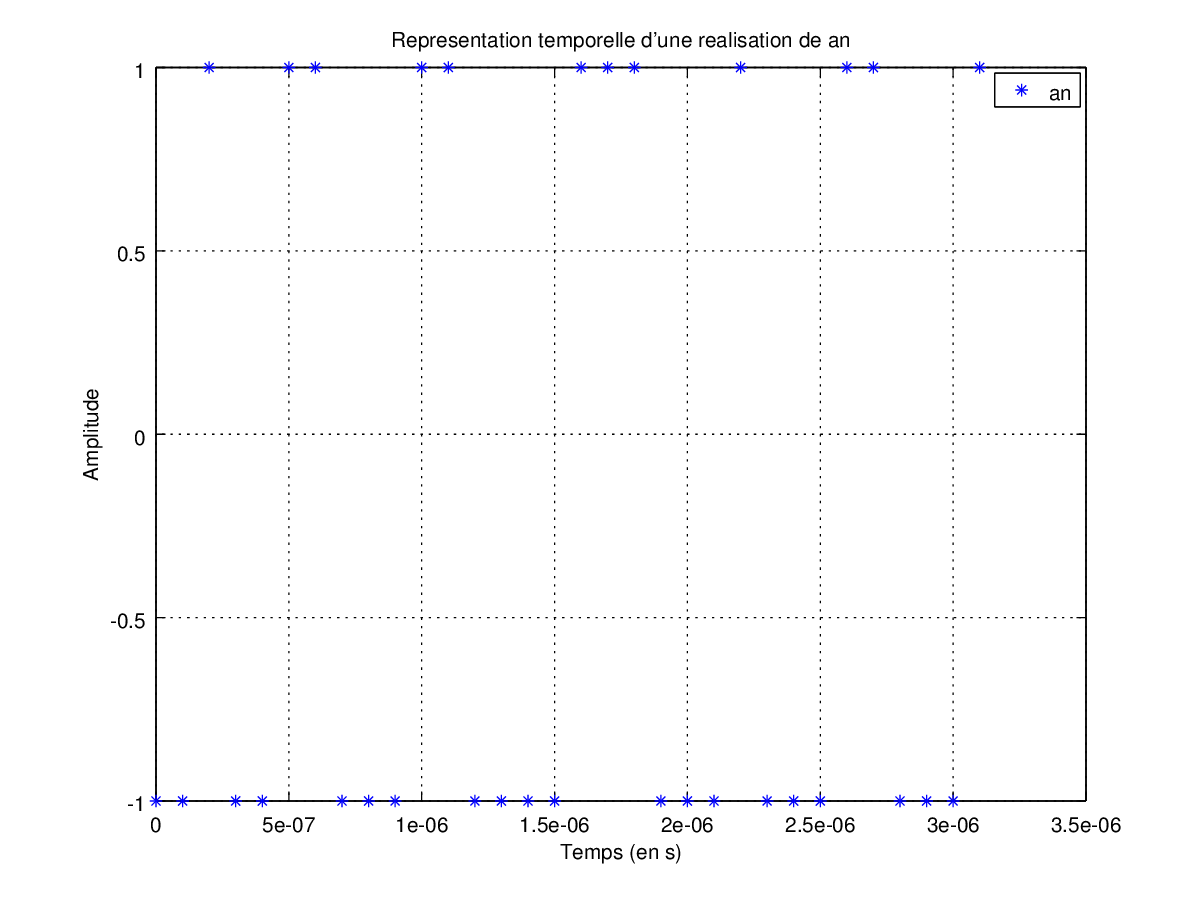
\includegraphics[scale=0.45]{ak_2.png}
\captionof{figure}{Représentation temporelle d'une réalisation de an}

\begin{lstlisting}
plot(real(an), imag(an), '*')
\end{lstlisting}

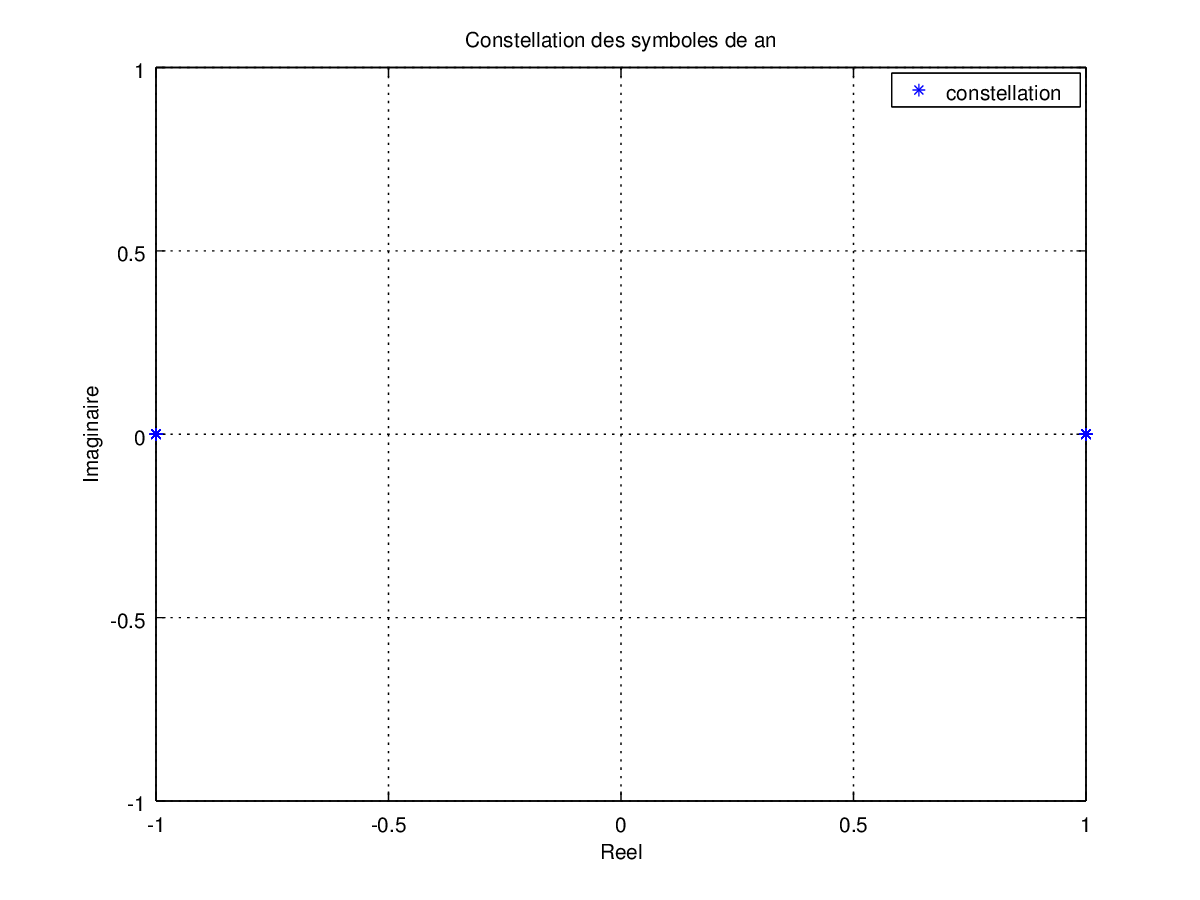
\includegraphics[scale=0.45]{constell_2.png}
\captionof{figure}{Constellation des symboles de an}
\end{center}


\section{Conversion numérique - analogique}
\subsection{Expansion - Question 1}

La durée du signal st peut s'écrire : NF/D.

\begin{center}
\begin{lstlisting}
N = 32;

F = 16;
st = zeros(1, N*F);
st(1) = F*an(1);
for k=1:1:length(an)-1
    st(k*F+1) = F*an(k+1);
end
\end{lstlisting}

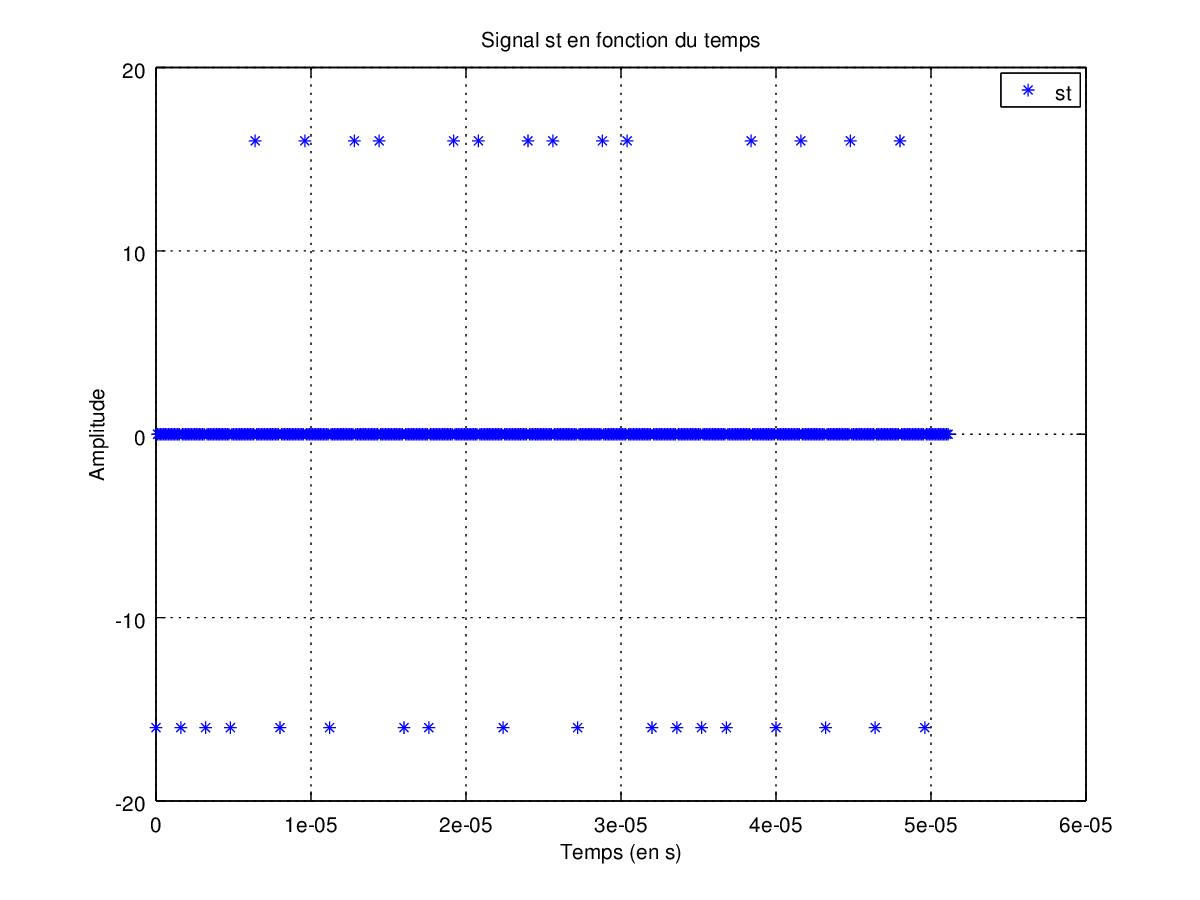
\includegraphics[scale=0.45]{st_3.png}
\captionof{figure}{Signal st en fonction du temps}
\end{center}

\subsection{Etude des filtres - Question 2}

\begin{lstlisting}
N = 32;

L = 8;
alpha = 0.5;
Te = T/F;
t_filtre = [0 : T/F : L*T -T/F];
\end{lstlisting}

\subsubsection{NRZ}

\begin{center}
\begin{lstlisting}
s_t = gen_filters2('nrz',t_filtre,T,F,L,alpha);
plot(t_filtre, s_t, '*')
\end{lstlisting}

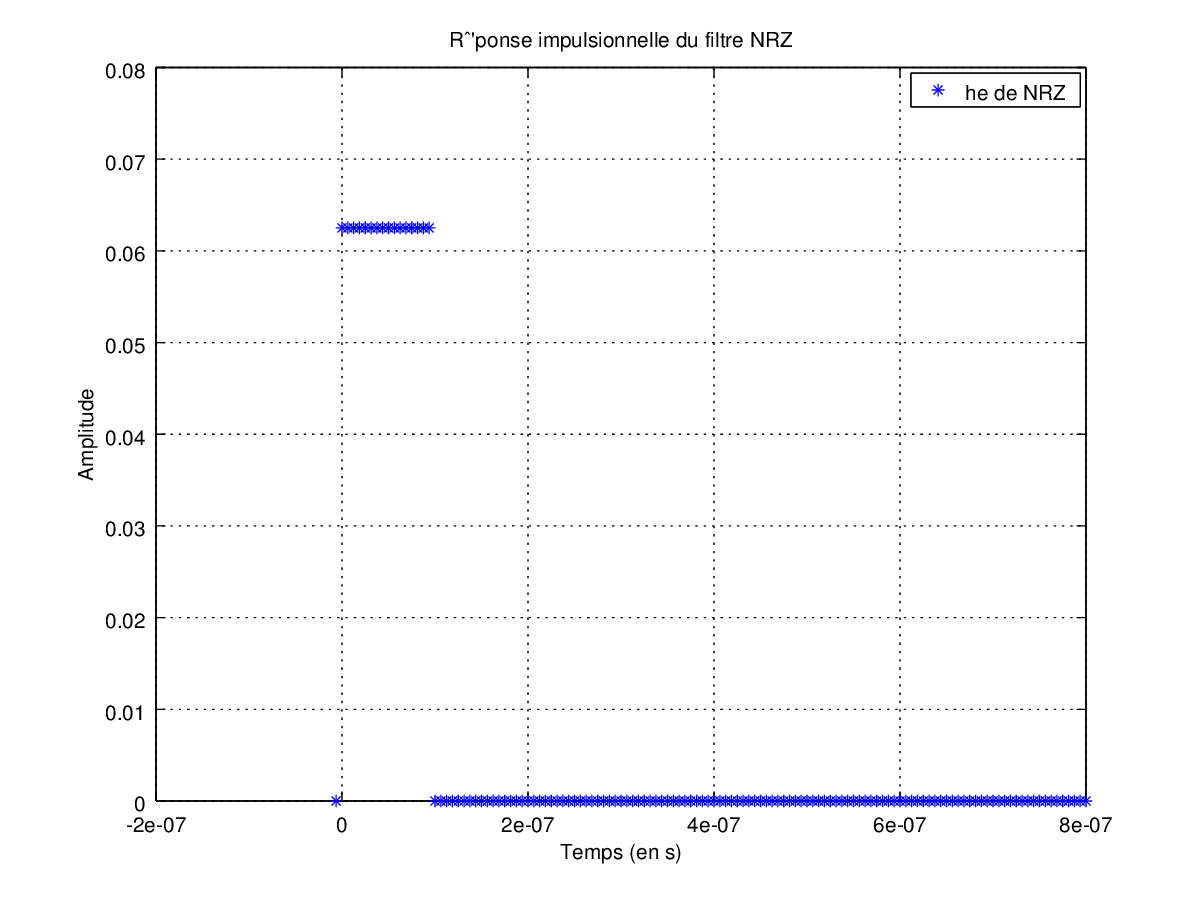
\includegraphics[scale=0.45]{NRZ_3.png}
\captionof{figure}{Réponse impulsionnelle du filtre NRZ}

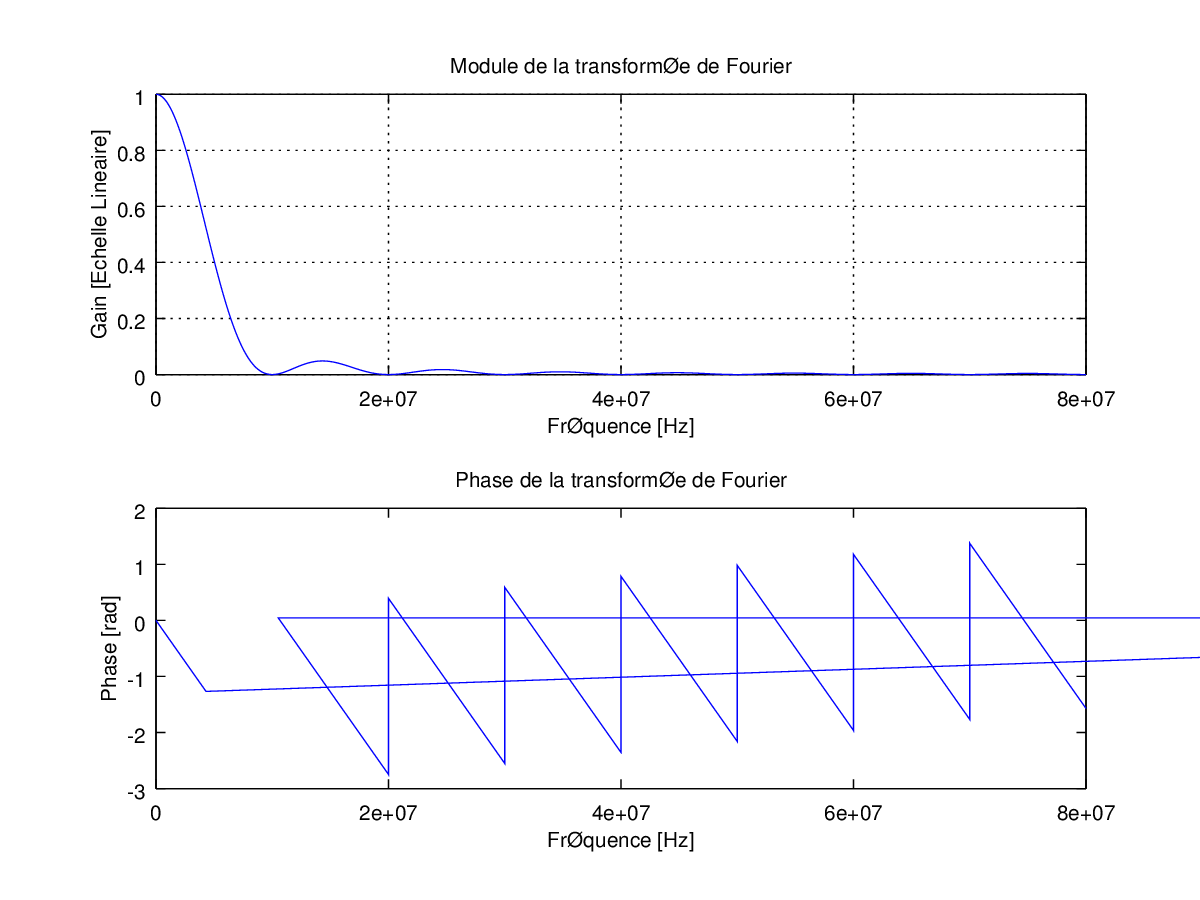
\includegraphics[scale=0.45]{NRZ_rep_3.png}
\captionof{figure}{Module de la transformée de Fourier de la réponse impulsionnelle du filtre NRZ}
\end{center}

\subsubsection{RZ}

\begin{center}
\begin{lstlisting}
s_t = gen_filters2('rz',t_filtre,T,F,L,alpha);
plot(t_filtre, s_t, '*')
\end{lstlisting}

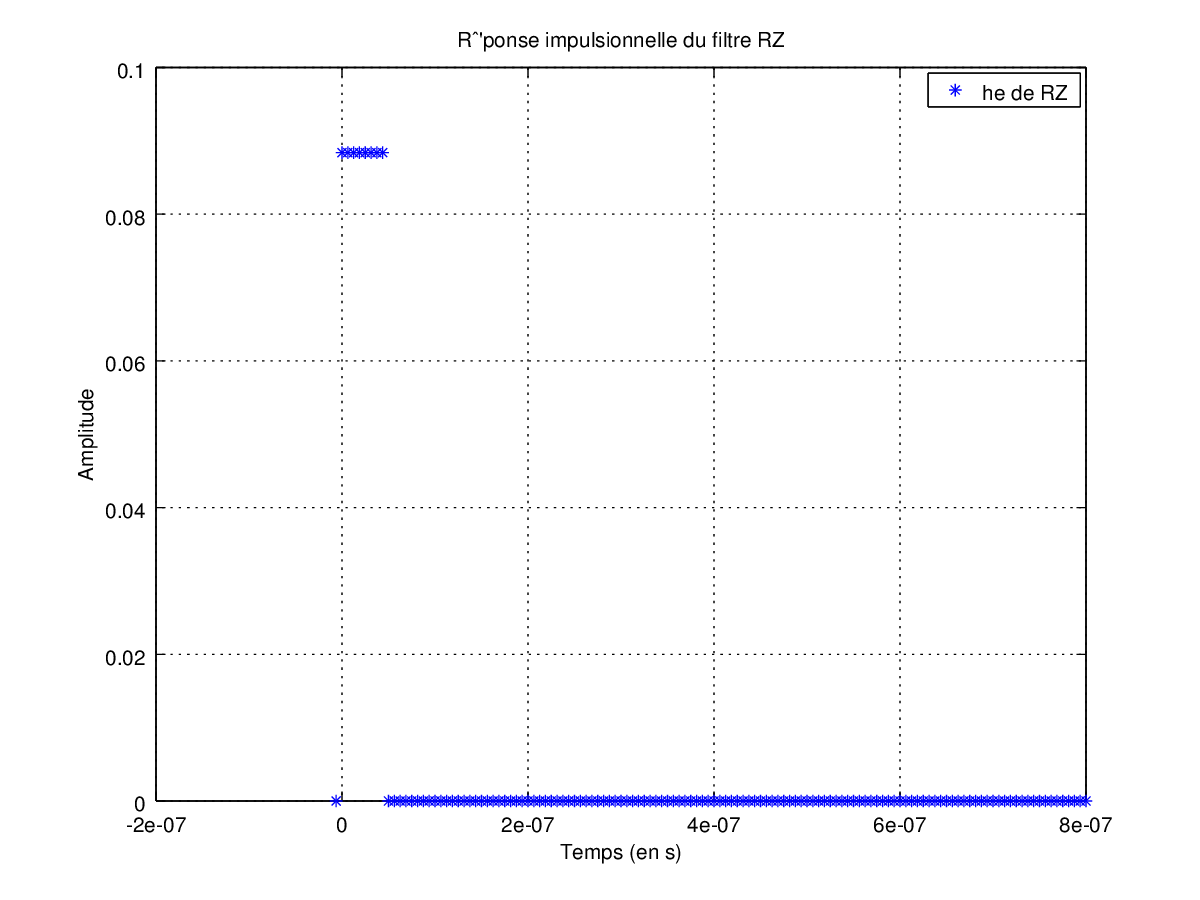
\includegraphics[scale=0.45]{RZ_3.png}
\captionof{figure}{Réponse impulsionnelle du filtre RZ}

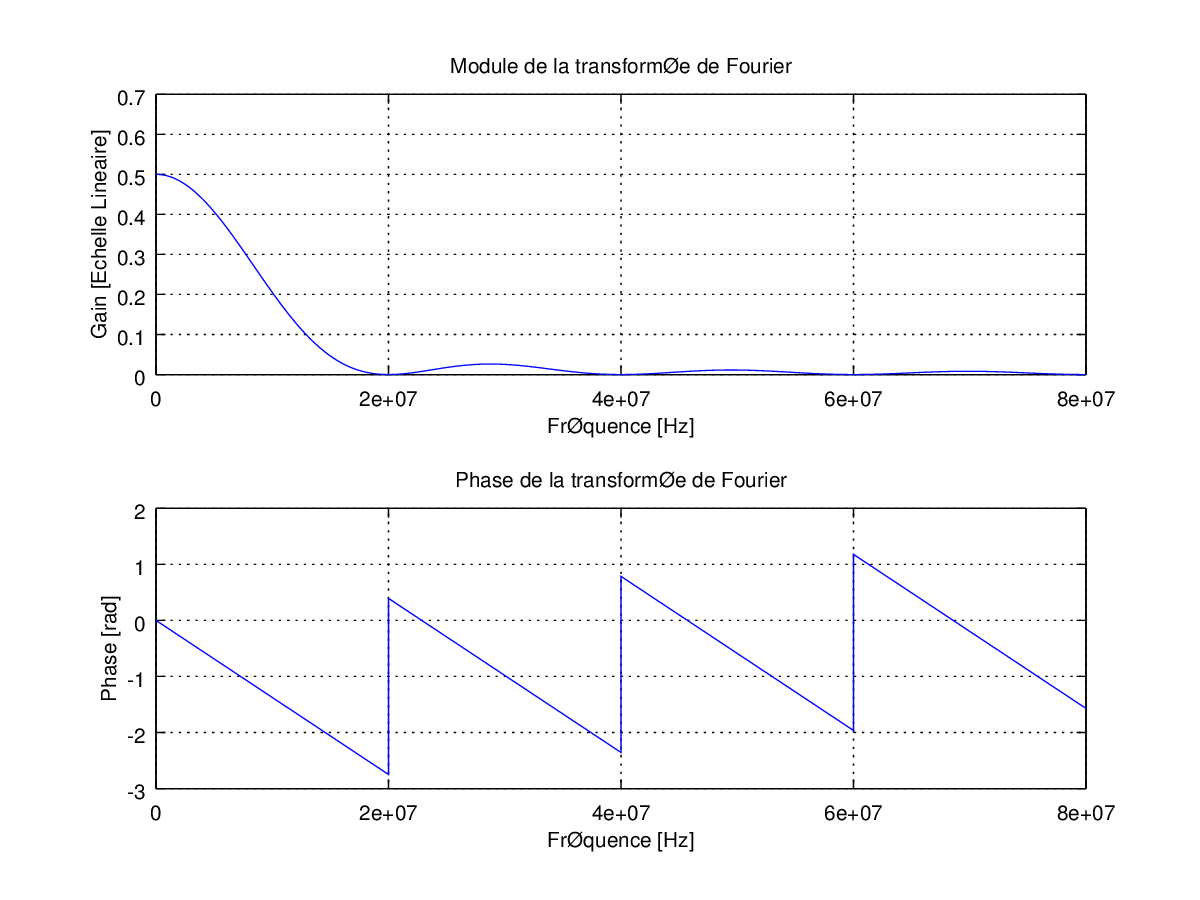
\includegraphics[scale=0.45]{RZ_rep_3.png}
\captionof{figure}{Module de la transformée de Fourier de la réponse impulsionnelle du filtre RZ}
\end{center}

\subsubsection{SRRC}

\begin{center}
\begin{lstlisting}
s_t = gen_filters2('srrc',t_filtre,T,F,L,alpha);
plot(t_filtre, s_t, '*')
\end{lstlisting}

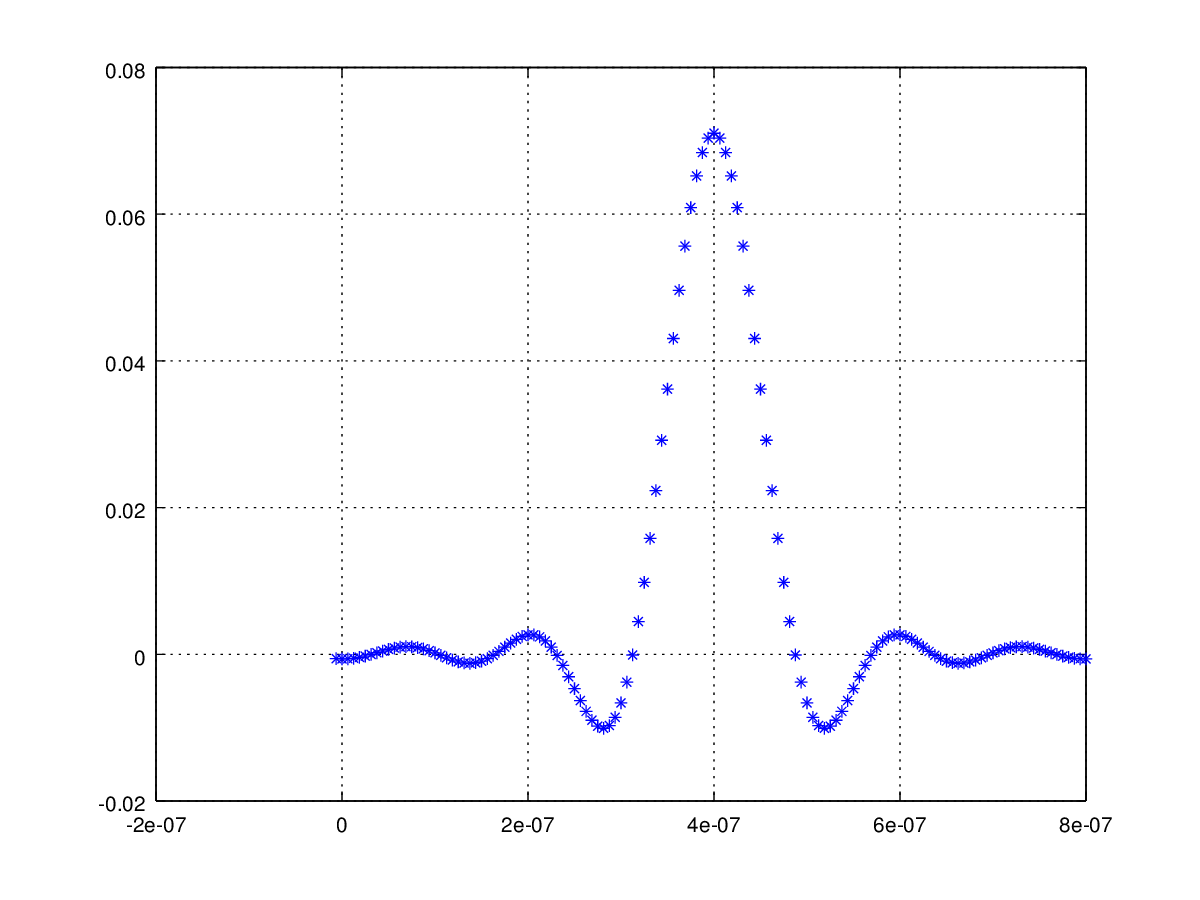
\includegraphics[scale=0.45]{SRRC_3.png}
\captionof{figure}{Réponse impulsionnelle du filtre SRRC}

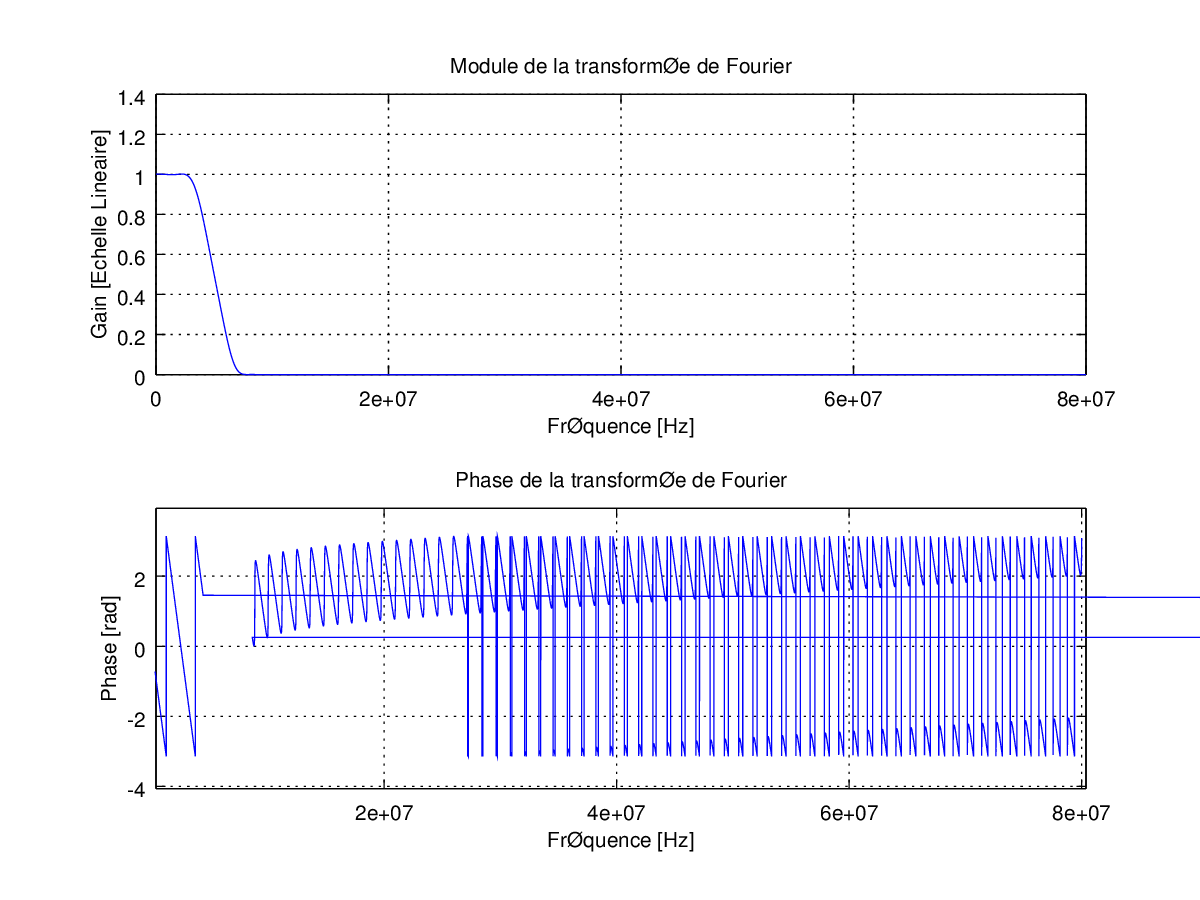
\includegraphics[scale=0.45]{SRRC_rep_3.png}
\captionof{figure}{Module de la transformée de Fourier de la réponse impulsionnelle du filtre SRRC}

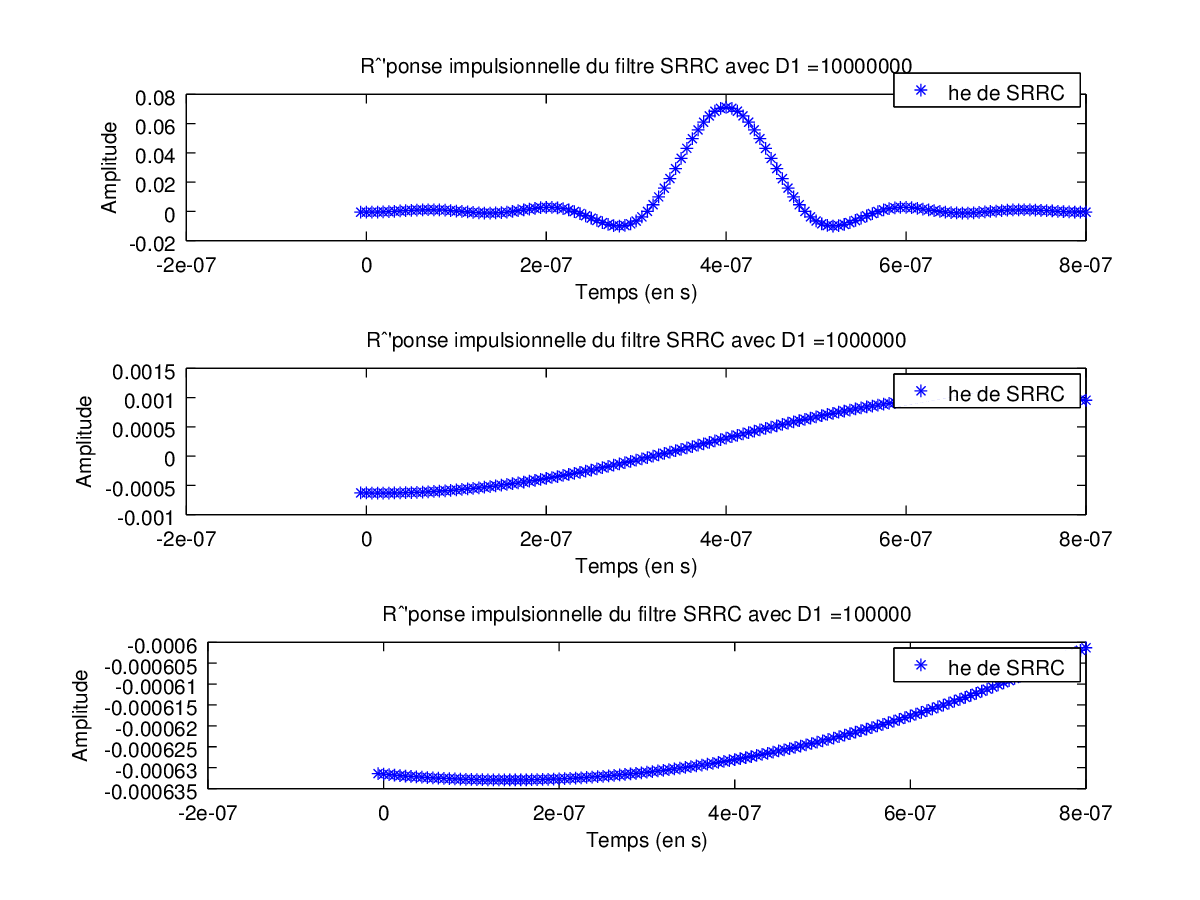
\includegraphics[scale=0.45]{SRRC_varD_3.png}
\captionof{figure}{Variation de la réponse impulsionnelle du filtre SRRC avec le débit}

Interêt de D : 

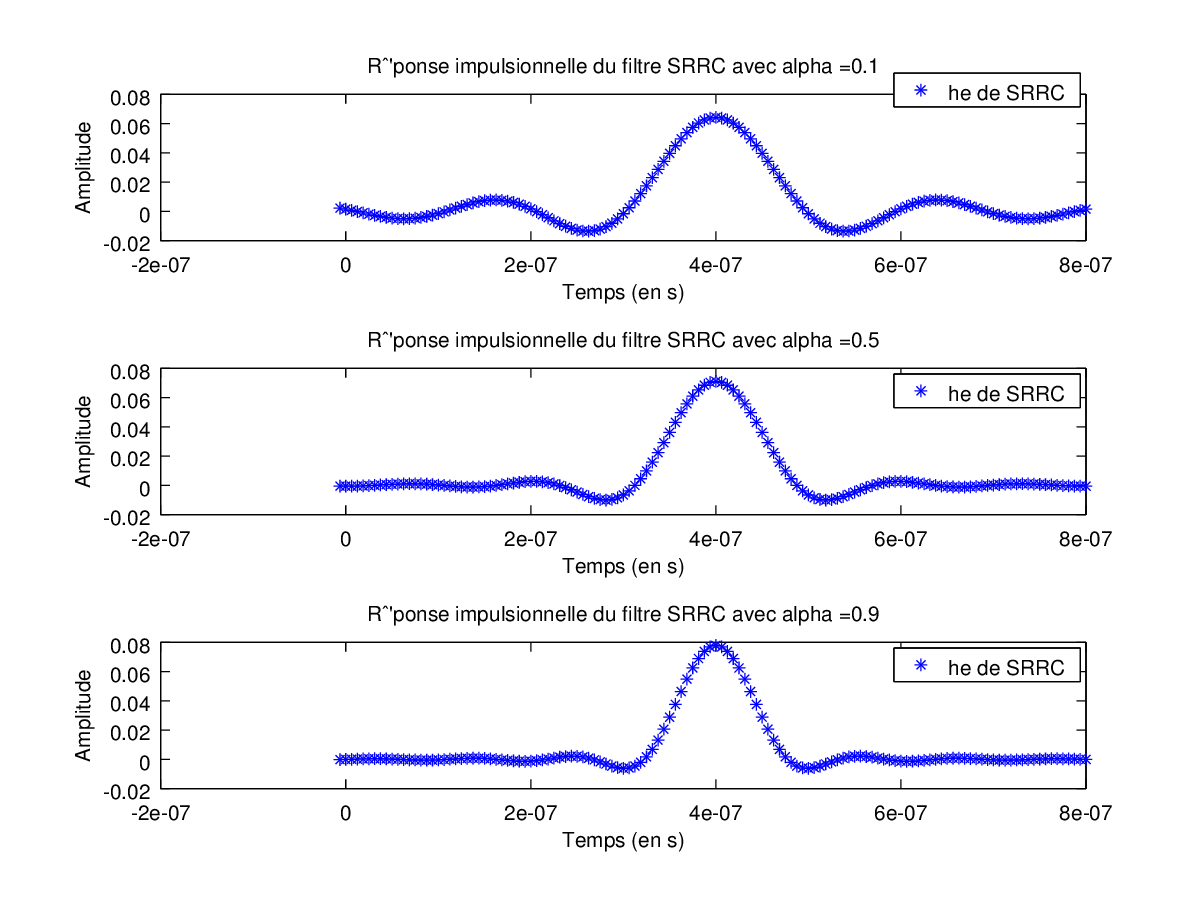
\includegraphics[scale=0.45]{SRRC_varAlpha_3.png}
\captionof{figure}{Variation de la réponse impulsionnelle du filtre SRRC avec alpha}
\end{center}

Interêt de alpha :

Est-ce logique d'observer une variation de phase linéaire avec la fréquence ?

\subsection{Mise en forme des symboles}

\subsubsection{Question 3}
\begin{center}
\begin{lstlisting}
N = 32;

t_x = -L*F*T/2 : T : (N*F)*T + L*F*T/2;
ht = gen_filters2('srrc',t_filtre,T,F,L,0.5);
xt = conv(st, ht);
figure; subplot(2,1,1); plot(t_s, st, '*');
subplot(2,1,2); plot(t_x, xt);
\end{lstlisting}

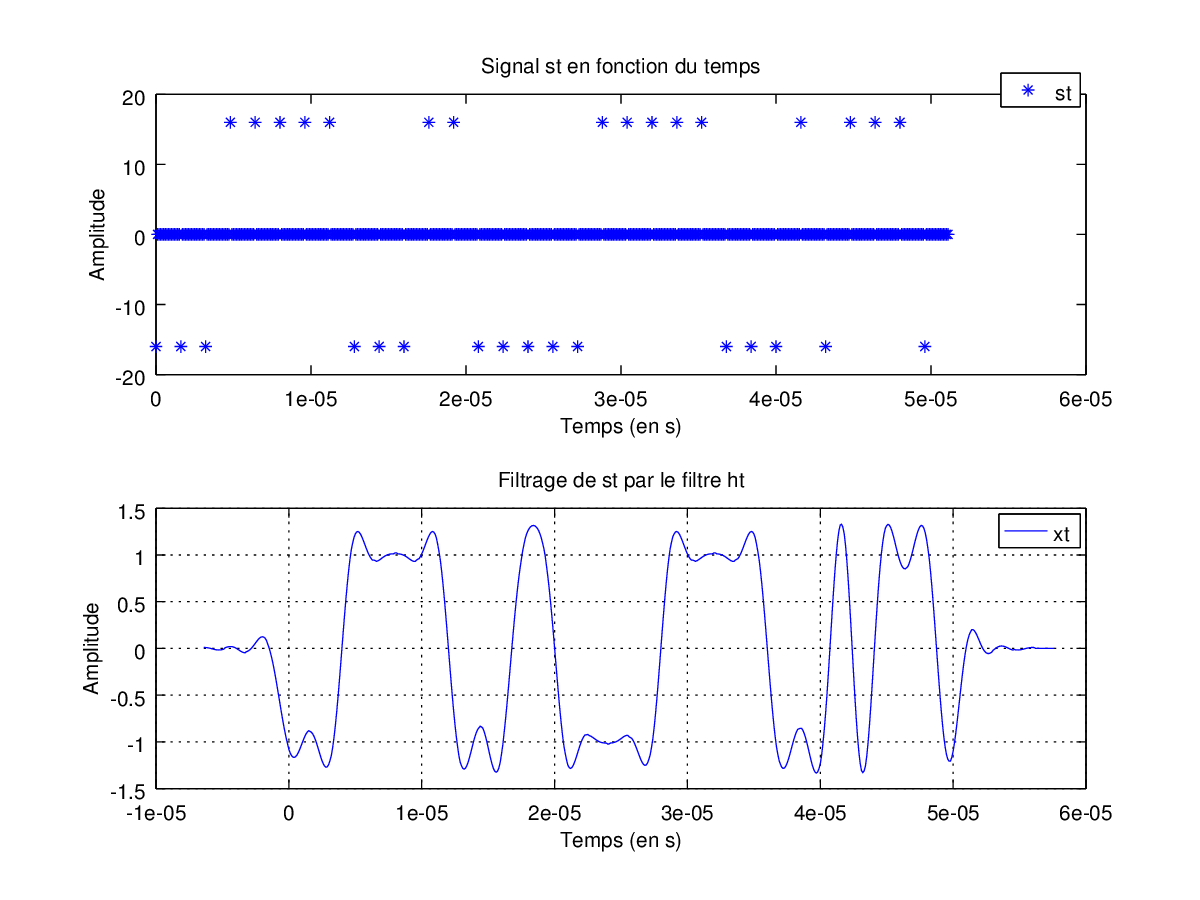
\includegraphics[scale=0.45]{conv_3_3.png}
\captionof{figure}{Signal st et son filtrage par ht en fonction du temps}

\begin{lstlisting}
length(st)
length(ht)
length(t_x)*T
length(t_filtre)*T
\end{lstlisting}
\end{center}

Résultats : ans =  512 (16*32)
ans =  130 (LF)
ans =    6.4100e-05 (cf ts)
ans =    1.3000e-05 (cf tfiltre)

\subsubsection{Question 4}
\begin{lstlisting}
N = 2048;

mean(xt.^2)
\end{lstlisting}

La puissance moyenne empirique du signal émis xt vaut 1. Ceci est cohérent avec la théorie car la variance vaut 1 et le norme carrée du filtre d'émission vaut 1/T (filtre normalisé).

\subsubsection{Question 5}

\subsubsection{Question 6}


\section{Ajout du bruit blanc gaussien - Question 7}

On sait que $sigman^{2}$ = $\frac{NoF}{2T}$
or P(xt) = $\frac{Eb}{T}$ d'où la formule $\frac{Eb}{N0}$ = $\frac{F}{2}$*($\frac{P(xt)}{sigman^{2}}$).



De plus, on a P(xt) = 1 ici, donc sigman² = f($\frac{Eb}{N0}$) avec f(x) = $\frac{F}{2x}$.

\begin{center}
\begin{lstlisting}
EbN0 = 100;

sigma_n = sqrt((F/2)/EbN0);
nt=sigma_n*randn(1,length(xt));
rt = xt + nt;
\end{lstlisting}

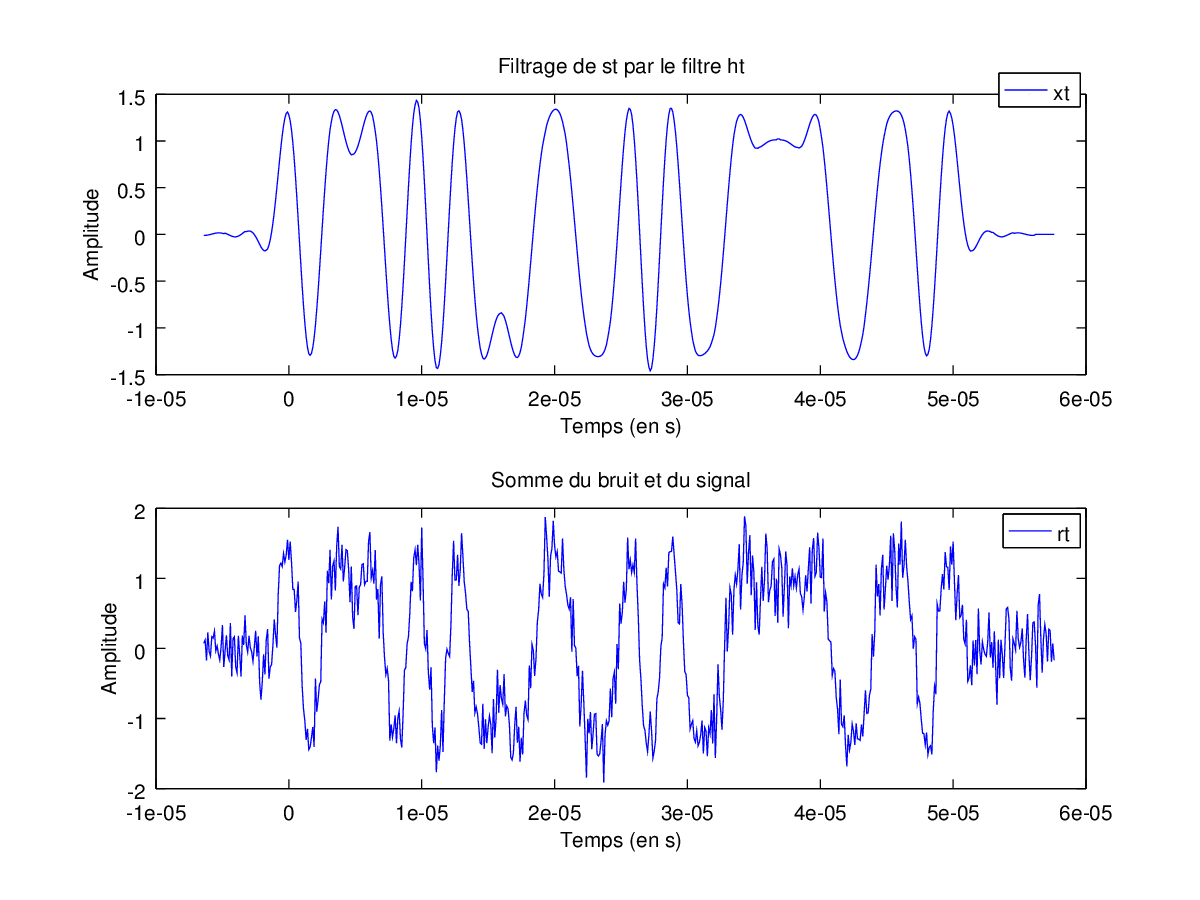
\includegraphics[scale=0.45]{signalBruite_7.png}
\captionof{figure}{Filtrage de st par le filtre ht et le même signal bruité}
\end{center}


\section{Conversion analogique - numérique}
\subsection{Filtrage adapté}
\subsubsection{Question 8}
Définition de filtre adapté : filtre de réception optimum permettant une rapport signal à bruit en sortie du FA bien échantilloné maximum et une probabilité d'erreur minimum.\\

\subsubsection{Question 9}

\begin{center}
\begin{lstlisting}
N = 32;

htr = fliplr(ht+L*T);
plot(t_filtre, ht, '*');
plot(t_filtre, htr, 'r+');
\end{lstlisting}

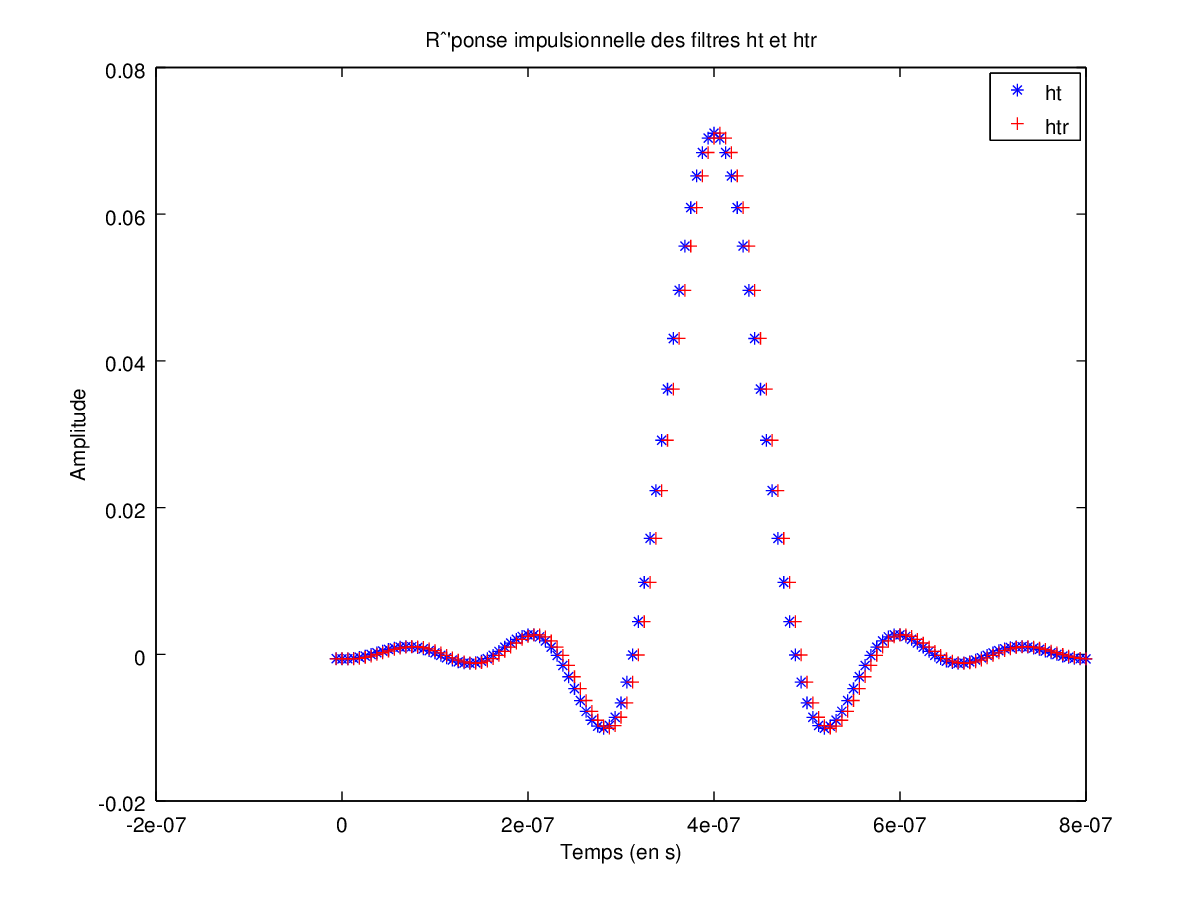
\includegraphics[scale=0.45]{ht_htr_9.png}
\captionof{figure}{Réponse impulsionnelle des filtres ht et htr}
\end{center}

Comme le filtre ht a une symétrie paire, le filtre adapaté associé sera le filtre ht (en considérant le décalage en temps). C'est ce qui se vérifie sur la figure ci-dessus.

\begin{center}
\begin{lstlisting}
pt = conv(ht, htr);

t_filtre_pt = [0 : T/F : 2*(L*T + T/F)];
figure; plot(t_filtre, ht, '*'); hold on;
plot(t_filtre_pt, pt, 'r+');
\end{lstlisting}

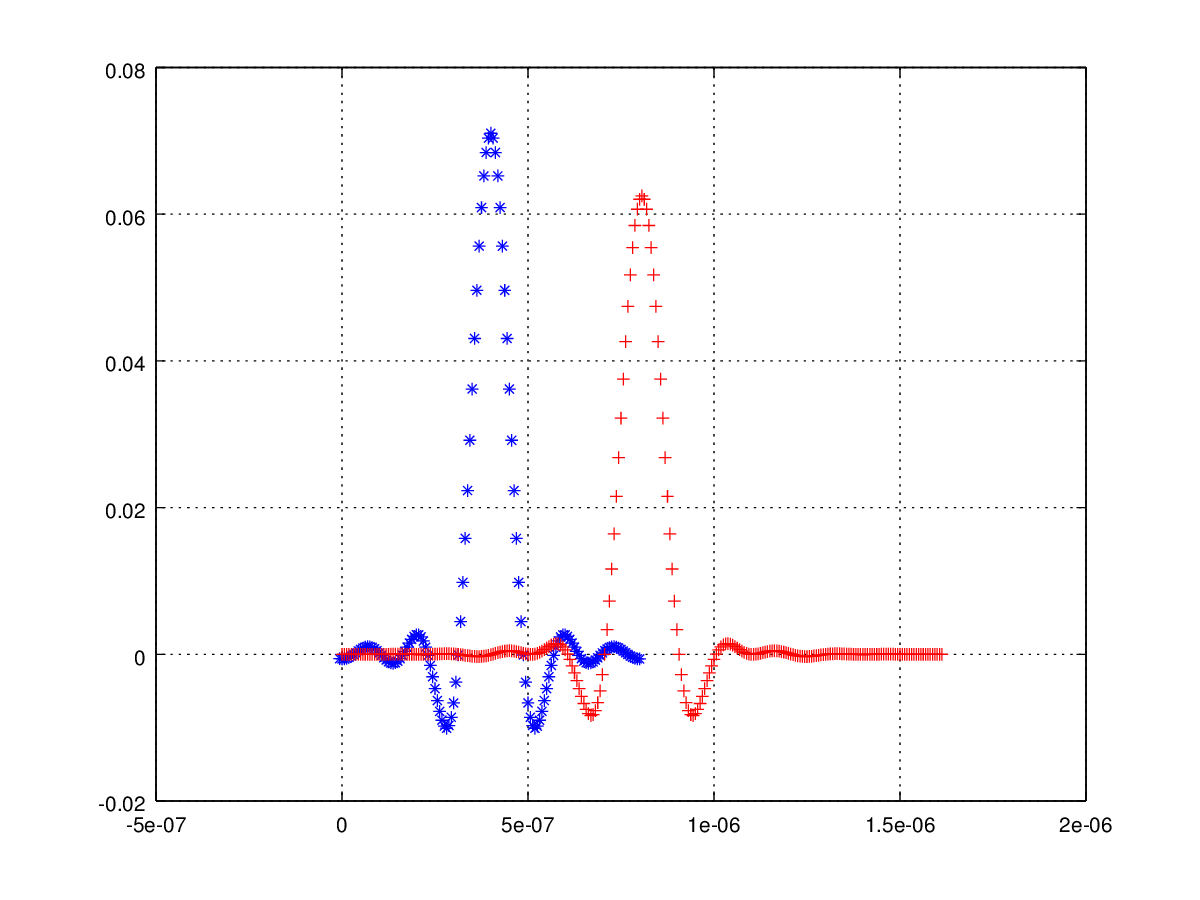
\includegraphics[scale=0.45]{ht_pt_9.png}
\captionof{figure}{Réponse impulsionnelle du filtre ht et du filtre adapté}
\end{center}

Pt est construit comme le retourné décalé de ht. Ici on a choisi LT comme décalage afin que le filtre équivalent émission-réception soit causal.\\
On sait que le vecteur temps t\_filtre\_pt vaut le double du vecteur t\_filtre par convolution.

\subsubsection{Question 10}

A l'aide de Matlab on fait créer un vecteur contenant les valeurs de pt prises en to + nTs avec to = L*T et Ts = T.

\begin{center}
\begin{lstlisting}
vect_result = zeros(1,17);

for k=1:1:8
  vect_result(9-k) = pt(round((L*T-k*T)/(T/F)));
  vect_result(9+k) = pt(round((L*T+k*T)/(T/F)));
end

vect_result(9) = pt(round((L*T)/(T/F)));

t_vect_result = [L*T - 8*T: T : L*T + 8*T];
plot(t_vect_result, vect_result, '*')
\end{lstlisting}

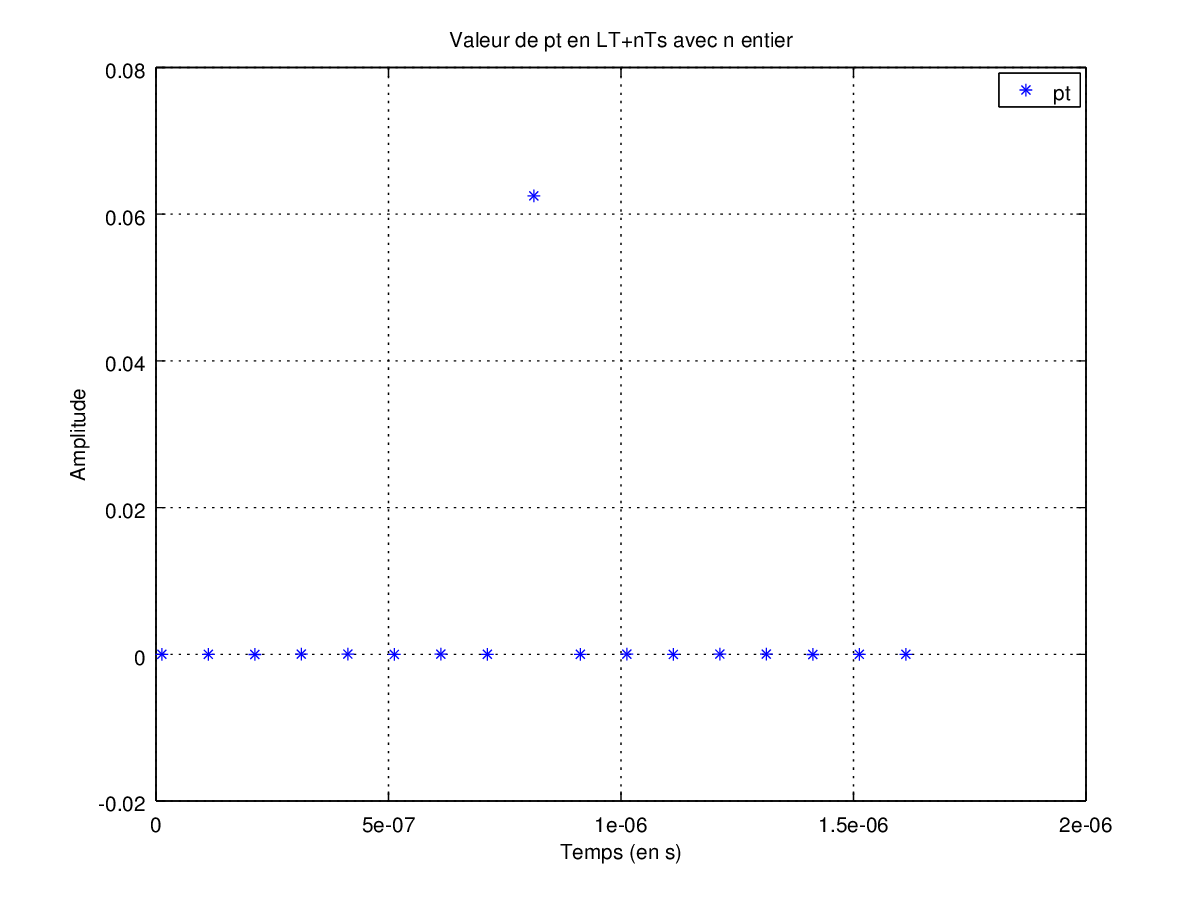
\includegraphics[scale=0.45]{pt_nyquist_10.png}
\captionof{figure}{Valeur de pt en LT+nTs avec n entier}
\end{center}

On voir que pour n <> 0 les valeurs de pt sont bien nulles. On ne peut pas transmettre sans IES car on ne peut atteindre une précision telle que pt aura une valeur nulle tous les to + nTs. On peut s'en approcher, et donc minimiser l'IES, en essayant de se rapprocher au maximum de 0.

\begin{center}
\begin{lstlisting}
t_y = -L*F*T : T : (N*F)*T + L*F*T + T;
yt = conv(rt, htr);
plot(t_y, yt, '*')
eyepattern(yt,T,F,32,1,1)
\end{lstlisting}

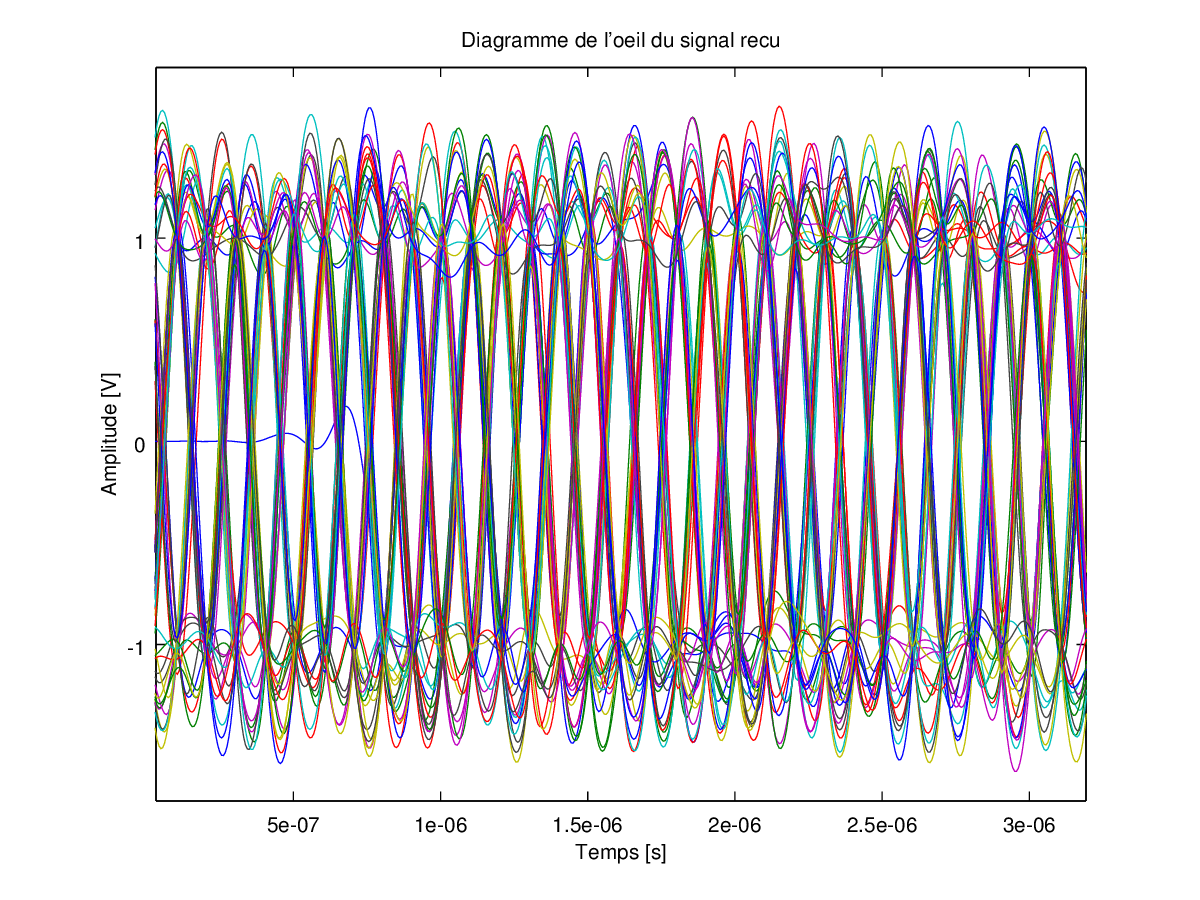
\includegraphics[scale=0.45]{oeil.png}
\captionof{figure}{Diagramme de l'oeil du signal yt}
\end{center}
\subsubsection{Question 11}

blablablablabla

\subsection{Décimation}

\subsubsection{Question 12}

cf cours

\subsubsection{Question 13}

\begin{center}
\begin{lstlisting}
t_y = -L*F*T : T : (N*F)*T + L*F*T + T;
yt = conv(rt, htr);

plot(t_x, xt); hold on; plot(t_y, yt, 'r');
\end{lstlisting}

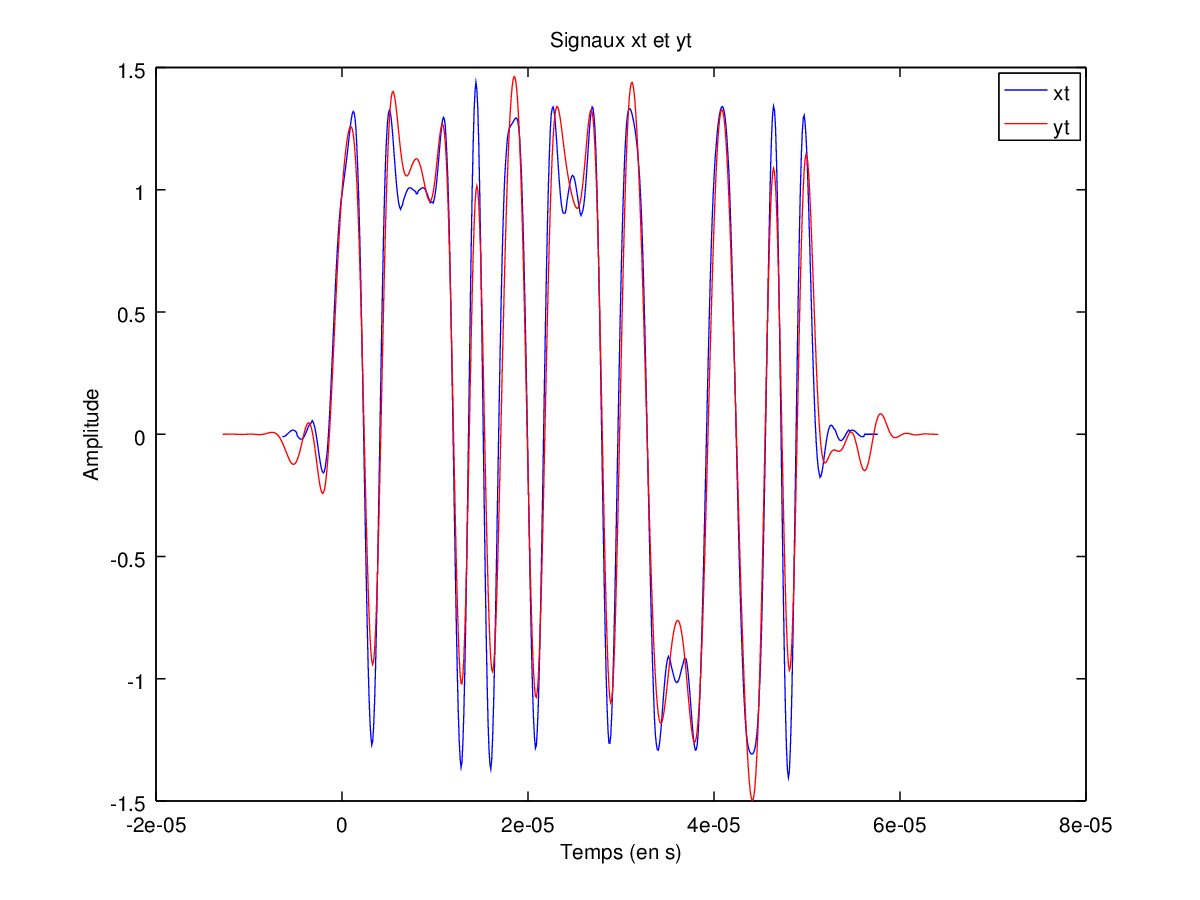
\includegraphics[scale=0.45]{yt_13.png}
\captionof{figure}{Signauc xt et yt}

\begin{lstlisting}
yk = [];

for k=1:1:length(yt)-1
    if mod(k, F) == 0 
      && -L*F*T + k*T >= 0 
        && -L*F*T + k*T < (N*F)*T
        yk = [yk F*yt(k)];
    end
end

t_yk = [0 : F*T : (N*F-1)*T];
figure; plot(t_s, st, '*'); hold on;
plot(t_yk, yk, 'r+')
\end{lstlisting}

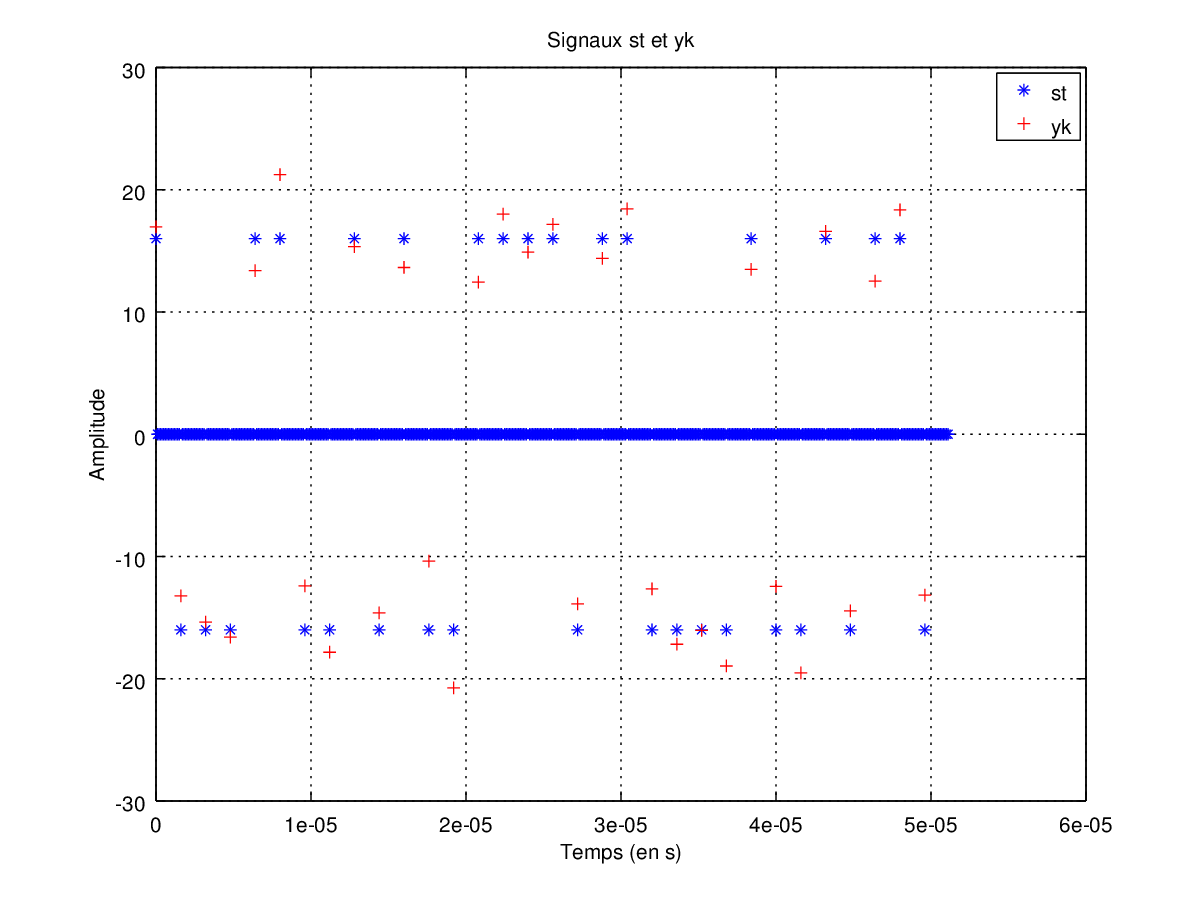
\includegraphics[scale=0.45]{yk_13.png}
\captionof{figure}{Signaux st et yk}
\end{center}

On vérifie grâce à la fonction length que le vecteur yk obtenu est bien de la même taille que an, soit 32.


\section{Prise de décision (demapping)}

On choisit comme seuil sigmaN (rapport avec le bruit)

\begin{center}
\begin{lstlisting}
bnF = [];

for k=1:1:length(yk)
    val = yk(k)/16;
    if val > 1 - 2*sigma_n
        bnF = [bnF 1];
    else
        bnF = [bnF 0];
    end
end

figure; plot(t_a, bn, '*'); hold on;
plot(t_a, bnF, 'ro');
\end{lstlisting}

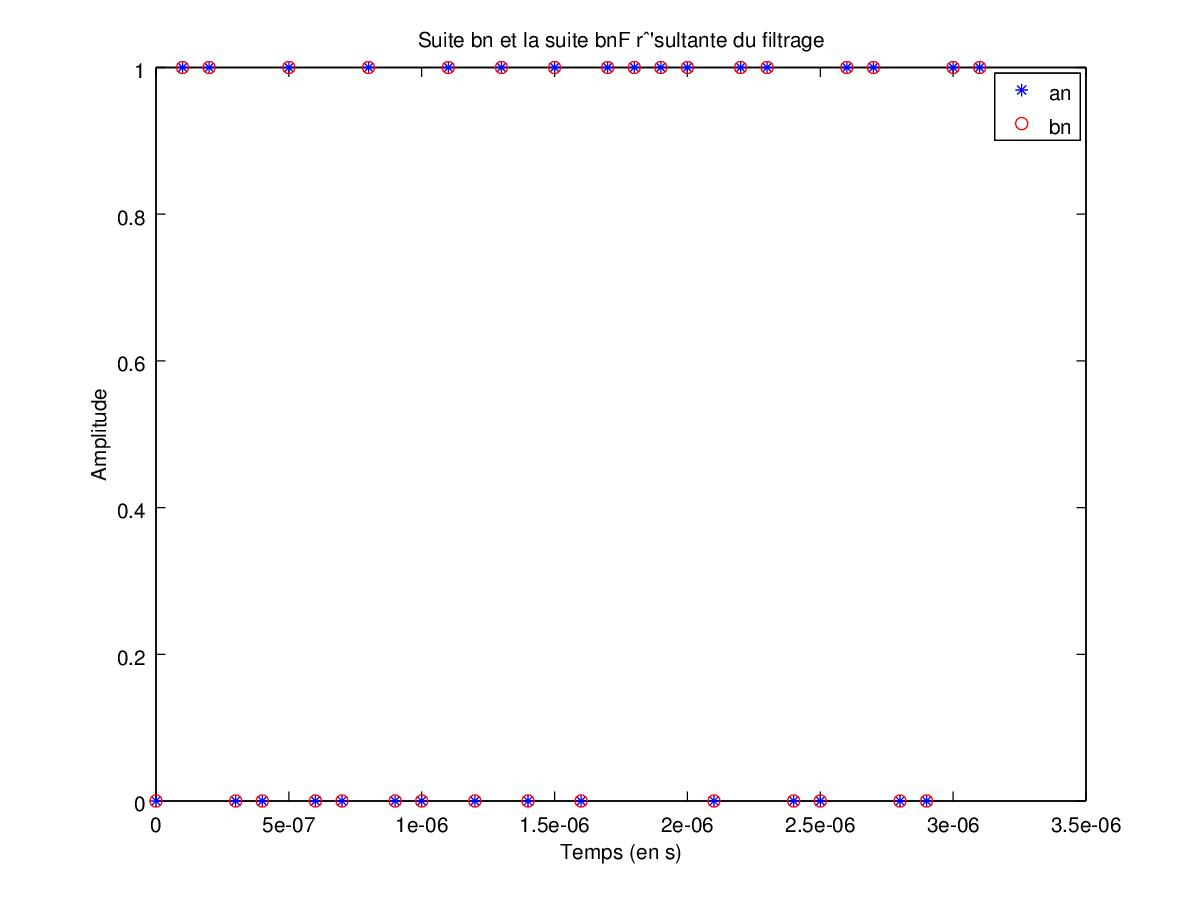
\includegraphics[scale=0.45]{bn_bnF_14.png}
\captionof{figure}{Signaux bn et la suite bnF résultante du filtrage}
\end{center}

\section{Calcul du taux d'erreur binaire}

\begin{lstlisting}
sum(xor(bn, bnF))/N
\end{lstlisting}

On trouve 0.027958 (avec N = 262144)

\section{Mesures de performances}


\begin{center}
\begin{lstlisting}
val_ebno = [50:200:20000];

vect_val_pratique = [];

for k=1:1:length(val_ebno)
    vect_val_pratique = 
      [vect_val_pratique teb(2048, val_ebno(k))];
end

plot(val_ebno, vect_val_pratique);
\end{lstlisting}

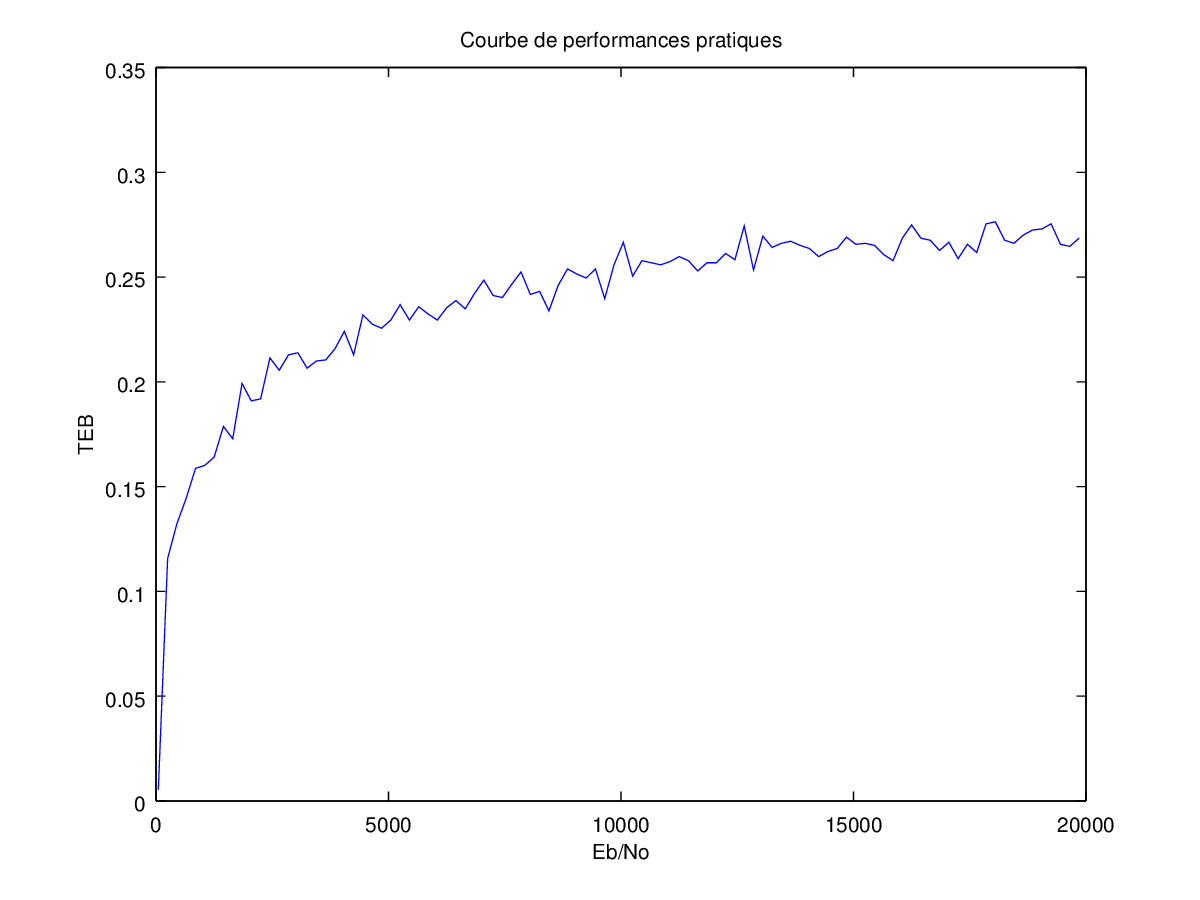
\includegraphics[scale=0.45]{performance_prat_8.png}
\captionof{figure}{Courbe de performances pratiques}
\end{center}

\section{Optionnel}
\subsection{Autres impulsions de mise en forme}
\subsection{Rapport signal à bruit sur la variable de décision}
\subsection{Analyseur de spectre}


\section{Conclusion}

\bibliographystyle{abbrv}
\bibliography{sigproc}  % sigproc.bib is the name of the Bibliography in this case
\nocite{*}

\balancecolumns
% That's all folks!
\end{document}
